\documentclass[12pt]{article}
\usepackage{graphicx,float}
\usepackage{amsmath,latexsym,amsfonts,amssymb,amsthm}

% \usepackage[utf8]{inputenc}
\usepackage[T1]{fontenc}
\usepackage[english]{babel}
% \usepackage[lithuanian]{babel}
\usepackage[letterpaper,top=2cm,bottom=2cm,left=3cm,right=1.5cm,marginparwidth=1.75cm]{geometry}
\renewcommand{\baselinestretch}{1.667} % 1.5 line spacing
\setlength{\parindent}{1cm}
\usepackage{mathptmx} % Times New Roman font

% Add . to (sub)sections everywhere (including table of contents)
\renewcommand{\thesection}{\arabic{section}.}
\renewcommand{\thesubsection}{\thesection\arabic{subsection}.}
\renewcommand{\thesubsubsection}{\thesubsection\arabic{subsubsection}.}

% Add dot lines to table of contents
\usepackage{tocloft}
\renewcommand{\cftdot}{\normalfont{.}}
\renewcommand{\cftsecleader}{\cftdotfill{\cftdotsep}}

% Page number on the bottom right
\usepackage{fancyhdr}
\pagestyle{fancy}
\fancyhead{}
\fancyfoot{}
\fancyfoot[R]{\thepage}

% For tables
\usepackage{array}

\usepackage{url}

\usepackage{caption}


\title{Course Work PS s7}
\author{Joris Plaščinskas}
\date{\today}


\begin{document}


\begin{center} %------TITLE PAGE------%
\thispagestyle{empty} % Remove page number

\includegraphics[scale=0.55]{images/MIF.png}
\end{center}
\vskip 20pt
\centerline{\bf \large \textbf{VILNIUS UNIVERSITY}}
\vskip 10pt
\centerline{\large \textbf{FACULTY OF MATHEMATICS AND INFORMATICS}}
\vskip 10pt
\centerline{\large \textbf{\MakeUppercase{Programų Sistemos \space study programme}}}

\vskip 80pt
\centerline{\Large Term Paper}
\vskip 20pt
\begin{center}{\bf \LARGE Software Architecture Assessment Criteria}
\end{center}
\begin{center}{\bf \Large Programų Architektūros Vertinimo Kriterijai}
\end{center}
\vskip 80pt

\begin{table}[h!]
    \centering
    \begin{tabular}{l l}
    Atliko: & 4 kurso Programų Sistemų 3 grupės studentas \\ 
            & Joris Plaščinskas \\
    Darbo vadovas: & Vasilij Savin, Lekt. \\
    \end{tabular}
\end{table}

\vfill
\centerline{Vilnius\textendash\the\year{}}
\newpage %------TITLE PAGE END------%


\tableofcontents %------CONTENTS PAGE------%
\thispagestyle{fancy} % Neccessary because table of contents resets page style
\newpage %------CONTENTS PAGE END------%


\section*{Introduction} %------INTRODUCTION PAGE------%
\addcontentsline{toc}{section}{Introduction}
The digital world is expanding rapidly. Providing new insights and possibilities, while also creating many software engineering challenges. As software systems grow in data consumption and complexity the relevance of a software architect role becomes more and more prominent. One of the key challenges in this field is understanding the systems and their properties. System properties are essentially answers to some question about a system. For example one question you could ask is: how well is the system able to handle sudden spikes in user activity? The answer should lead you to the elasticity characteristic. Understanding the questions you can ask about a system and the answers to them is at the heart of this term paper.


% Relevance:
% Software system criteria and metrics
\section{Term Paper Objective}
The objective of this term paper is to provide an overview of software system assessment criteria and metrics. The following tasks were derived to help achieve this goal:
\begin{itemize}
    \item Structure the overview of metrics and criteria around 3 abstraction levels from the C4 model: software system, container and module.
    \item Give an overview of existing quality models and relate each criteria/metric to quality characteristics.
    \item Do case studies to provider deeper insight.
\end{itemize}

% \item Investigate wether modularity metrics can be applied to 'modern' code.
% \item Provide methods for assessing containers.
% \item Provide a summary table in the results and conclusion section.
% \item Ground statements on scientific literature and articles.
% Most of this paper will be an overview of software engineering literature and various metrics that help assess a software system. The paper is structured around the C4 model - first the module level metrics and criteria are analyzed, then container level and finally software system level. In the results and conclusion section the author aims to provide a framework for evaluating software systems.
\newpage %------INTRODUCTION PAGE END------%


%------MAIN CONTENT------%
\section{Software Architecture and it's Components}
Before analysis, we first need to establish what the title of this paper means i.e. what do phrases "software architecture" and "assesment criteria" imply. "Assesment criteria" is easy, this phrase simply asks the question: what are the properties of something (in this case software) and how can we measure them. The term "software architecture" however, is a lot harder to define. There are many diffrent interprations for software architect's role across the industry. For example a software architect in organization A might work on requirements and solution design, while software architect in organization B may be responsible for implementing technological and organizational change. Very often architecture is associated with the structure of a software product, such as: a deployment diagram, or the logical grouping of code into modules. But in reality the software architect's role encompasses much more. The author of this paper prefers the definition given by Mark Richards and Neal Ford in their book about software architecture \cite{RF20}. They state that software architecture mainly consists of these four things:
\begin{itemize}
    \item Structure - the style or type that the system is implemented in, for example layered or micro services.
    \item Architecture characteristics - the success criteria of a system. Characteristics can be things like: system performance, availability, scalability, reliability, etc.
    \item Architecture decisions - are rules for how the system should be constructed. For example an architecture decision could be a choice of a development language.
    \item Design principles - are similar to architecture characteristics, but they serve more as guidelines rather than a hard rule.
\end{itemize}
In many cases architecture characteristics can be expressed in terms of some metric that can be either measured or evaluated subjectively. Architecture characteristics and metrics will be the main focus of this course work. So coming back to the paper's title: "software architecture assesment criteria" - there could be multiple interpretations of this. For example one could write a paper about different diagram types and claim that diagrams allow for assesment of the architecture, however from the authors point of view that would be considered visualizing rather than assesing. Another angle could be that in order to evaluate the architecture one must see how the architected system performs and how it's built. The author prefers the later definition. In this context the title could also be rephrased to: "software system assesment criteria from the perspective of architecture". We have come to a good understanding of the title, but we also introduced a new term - software system. Data driven applications are the most common type of a software system. But that's certainly not the only type of software. For example internet access on a plane is also a great software engineering challenge. One of the problems that the engineers had to solve is managing the internet consumption for each passenger. The passengers would need to connect to wifi and log into a website that tracks usage. Only then would the passenger have access to the internet. This is intresting, because the website could be hosted inside the plane or somewhere on the ground. This decision greatly impacts the characteristics and behaviour of a system. The main idea of this paragraph is that a software system is a lot more than just software. Also software exists on many different levels. For example, should a data warehouse be considered a software system or something else? Can a simple console tool be considered a software system? The author tries to provide an answer to these questions in the subsection below.

\subsection{C4 Model}
C4 model developed by Simon Brown provides a great answer to this question \cite{Bro11}. C4 is just a set of four hierarchical definitions, that states that - a software system is made up of containers, a container is made up of components and components are made up of code.
\begin{itemize}
    \item Software system is the highest level of abstraction and describes something that delivers value to it's users, whether they are human or not. Each organization will have different interpretation of this term, but usually this is something that a single development team delivers. Some examples of software systems are: a web shopping application, an anti money laundering system, some data warehouse, etc.
    \item Container represents the smallest separately deployable unit (program). A container is something that needs to be running for the overall software system to work. Some common examples of containers are:
    \begin{itemize}
        \item Server-side web application - a .NET service API.
        \item Database - any database instance like PostgreSQL, Microsoft SQL server, MongoDB, etc
        \item Client-side web application.
        \item File system - for example a network attached storage instance in AWS.
    \end{itemize}
    Note that, a full web application would not be considered a container, because usually at-least a database, a service API and front-end server are needed.
    \item Component (aka. module) is something that containers are made up of and is only applicable to containers that are built using code i.e. not a database. Component is essentially a logical grouping of code which can be in the form of a name space or package. Later in this paper the author instead uses the term module.
    \item Code is the actual code that powers the software system - the classes, the methods, configuration items, etc.
\end{itemize}
\newpage


\section{Modularity}
Probably one of the most important and frequently talked about topic in computer science is modularity. Module is a logical grouping of code, that can be used in conjunction with other modules to create some functionality. Programming languages feature many tools to implement modularity, such as classes, packages, namespaces, etc. but all of these fall under the abstraction of modularity. From the architectural point of view modularity is very important, because it enables for easy changes and makes the system more reliable. Many different metrics have been derived to evaluate modularity. For example cohesiveness is a metric that evaluates how well each procedure fit's together in one module. This is the type of metric that is hard to evaluate automatically, because it highly depends on the context. Many software architecture metrics require manual subjective evaluation. However some don't, for example the average request response time is a very objective metric and can be evaluated automatically. In the subsequent sub-sections the author provides a few metrics that are described in the book "Fundamentals of Software Architecture: An Engineering Approach" \cite{RF20}.

\subsection{Cohesiveness}
As described above, cohesiveness is a metric that evaluates how well a module groups the code. There are many different ways that a module can be cohesive. For example a module can be functionally cohesive if all parts of the module are related and the module contains everything essential to function. Or a module can be logically cohesive if all of the data within the module is logically related, but not functionally. For example an input/output library that groups many procedures together, which do not depend on each other is logically cohesive. Given the nature of cohesion, evaluating it usually comes down to manual work. However an LCOM formula can help indicate lack of cohesion:
\[
\text{LCOM} = 
\begin{cases} 
P - Q, & \text{if } P > Q, \\
0, & \text{otherwise},
\end{cases}
\]
$P$ is the number of methods that do not share any member fields, $Q$ is the number of methods that share a member variable. The LCOM metric can help architects find classes that are incidentally coupled.

\subsection{Coupling}
Two very simple, but useful metrics are afferent (incoming) and efferent (outgoing) relationship count. Most development platforms show afferent coupling count next to a method or class. By using efferent and afferent metrics you could derive the instability of a module:
\begin{equation}
I = \frac{C^e}{C^e + C^a}
\end{equation}
Here, $C^e$ represents efferent coupling count and $C^a$ represents afferent coupling count. The instability metric essentially tells us how much a module depends on other modules. A module that is highly dependent on other modules is more likely to break after changes to code base occur.

\subsection{Abstractness}
Modules that contain a lot of abstract code (abstract classes, interfaces, function definitions) are hard to learn. Abstractness metric is the ratio of abstract code unit's to concrete implementation:
\begin{equation}
A = \frac{\sum m^a}{\sum m^c}
\end{equation}
$m^a$ and $m^c$ here could mean abstract and concrete lines of code count.

\subsection{Distance from the Main Sequence}
Having some abstractness and instability in a module is actually good. Abstract constructs allow for polymorphism and code reuse. While high instability just means that a module has many dependencies. Code that is not abstract and that does not take advantage of other modules is very hard to manage and understand. While code that is very abstract and has many dependencies might be equally difficult to understand. The "distance from the main sequence" addresses the balance between these two metrics.
\begin{figure}[H]
    \centering
    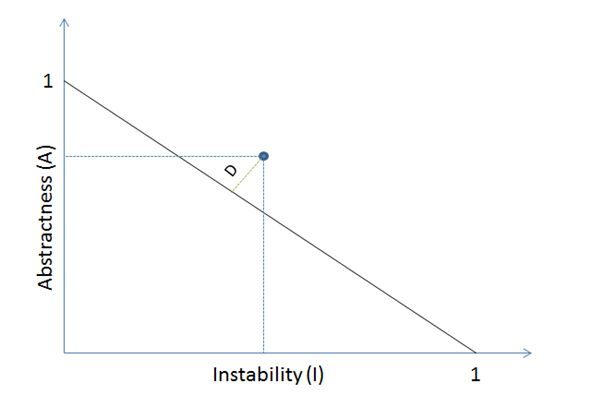
\includegraphics[width=0.7\textwidth]{images/dfms.jpg}
    \caption{Distance From Main Sequence from \cite{Mar15}.}
    \label{fig:dfms}
\end{figure}
In all normal cases instability and abstractness $\in [0, 1]$. In Figure~\ref{fig:dfms} a line is drawn between the two maximum values. All points on that line are considered to have an ideal relationship between abstractness and instability. A projection to the line from the actual value is the distance from main sequence metric. Area way above the line is considered to be the zone of uselessness, because code that is too abstract is difficult to use. On the contrary the area in the bottom left is considered the zone of pain, because code with not enough abstraction is hard to understand and maintain.

\subsection{Cyclomatic Complexity}
Cyclomatic complexity is another code metric that was developed by Thomas J. McCabe in 1976 \cite{Mcc76}. Cyclomatic complexity measures the number of independent paths through a program or a procedure. It can be used to determine the stability of the code. High cyclomatic complexity code bases are hard to understand and test. Figure~\ref{fig:cyclomatic-complexity} represents a program as a flow graph, where each node can be thought of as a statement. Any conditional statements (if statements, conditional goto statements, loops) split flow of the program by adding more than one edge.
\begin{figure}[H]
    \centering
    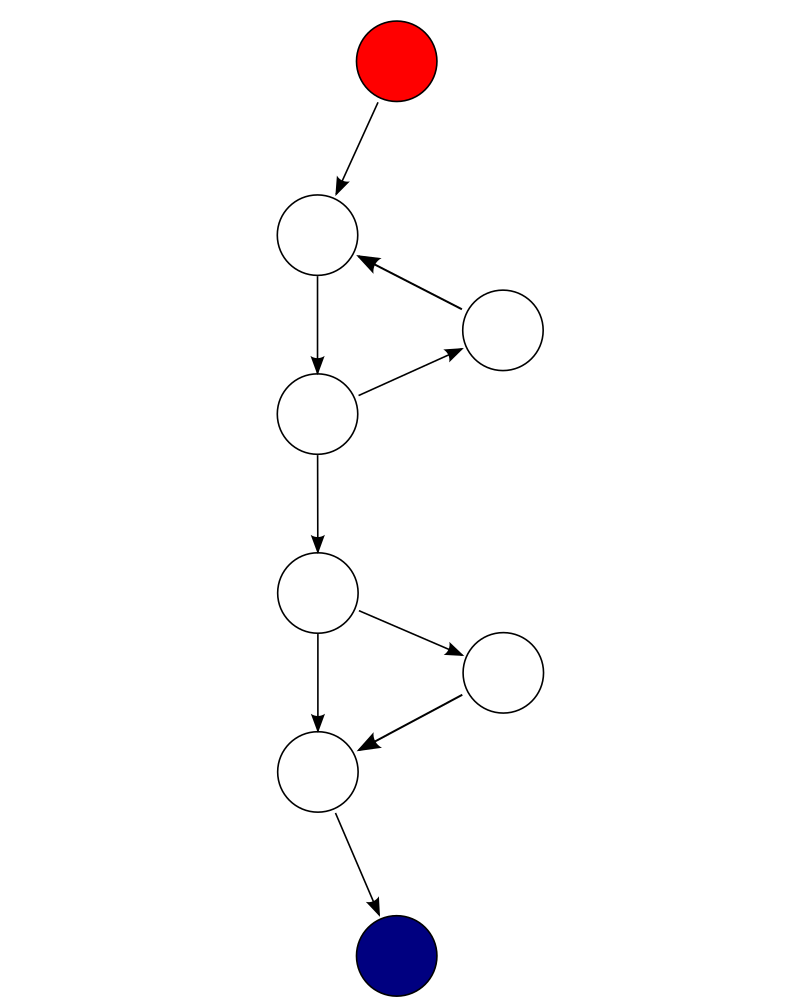
\includegraphics[width=0.3\textwidth]{images/cyclomatic-complexity.png}
    \caption{Program represented as a flow graph from Wikipedia \cite{Mcc76}.}
    \label{fig:cyclomatic-complexity}
\end{figure}
The formula for calculating Cyclomatic complexity is: $M = E - N + 2P$, where E - is the number of edges, N - is the number of nodes and P is the number of connected components (functions that don't depend on one another). 

\subsection{Modularity Metrics In Practice}
A very natural question to ask is: are modularity metrics applicable to modern frameworks and distributed systems? Most metrics that can be used to evaluate code's modularity were developed long ago in the days of c++. Since then many new programming constructs have been created, such as: middle-ware pattern, dependency injection frameworks, generic classes, etc. Also, modern systems are much more distributed (and not directly coupled through code). To assess wether or not these metrics can be applied to modern systems we will look at a few examples of modern code.
\subsubsection{Python Front-end Server Example}
Figure~\ref{fig:simple-python-server} shows a simple web application written in Python using a modern framework called Flask. The web page has a home page that is linked to the contacts page. The Contacts page makes an API call to the street endpoint to retrieve the address. Even though the example program is small, it uses the same structural constructs as any bigger commercial application would use. Flask framework takes over the execution of a program and routes requests using function decorators, however this doesn't stop us from calculating the cyclomatic complexity, because it can be calculated separately for each function.
\begin{figure}[H]
    \centering
    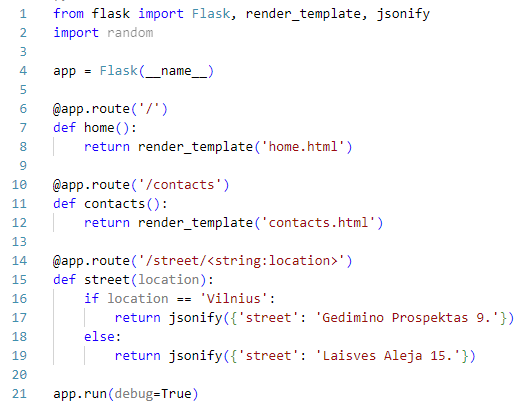
\includegraphics[width=0.6\textwidth]{images/simple-python-server.png}
    \caption{Web server written in Python.}
    \label{fig:simple-python-server}
\end{figure}
Calculating cyclomatic complexity for each function separately gives us: 1 for home route, 1 for contacts route, and 2 for phone route. However, notice that both cyclomatic complexity and other metrics defined above don't capture the coupling when front-end makes an API call to fetch the street i.e. they don't extend to distributed systems. These metrics also don't apply to the process of Flask framework building the HTML templates, which can also fail. In essence, cyclomatic complexity can be applied to modern frameworks like Flask, but they don't cover every aspect of it. A mission critical API is one of the best use cases for cyclomatic complexity metric, as it allows to pin point the most complex endpoints, which are most likely to fail.

\subsubsection{.NET API Example}
Figure~\ref{fig:dotnet-example} shows an API endpoint that is written using C\# ASP.NET Core. This example introduces two new modern constructs that are handled by the framework: middle-ware and dependency injections. Middle-ware in .NET framework essentially adds prior method calls to the stack, before finally calling the endpoint method, but that does not affect the cyclomatic complexity metric as it is calculated for each method separately. Same can be said about dependency injection - cyclomatic complexity is calculated based on the internal control flow of each individual method. That means even though the method calls an abstract interface method it does not change it's internal control flow. In essence, both dependency injection and middle-ware add complexity to the code base, which needs to be tested separately, but they don't affect the use of cyclomatic complexity metric.
\begin{figure}[H]
    \centering
    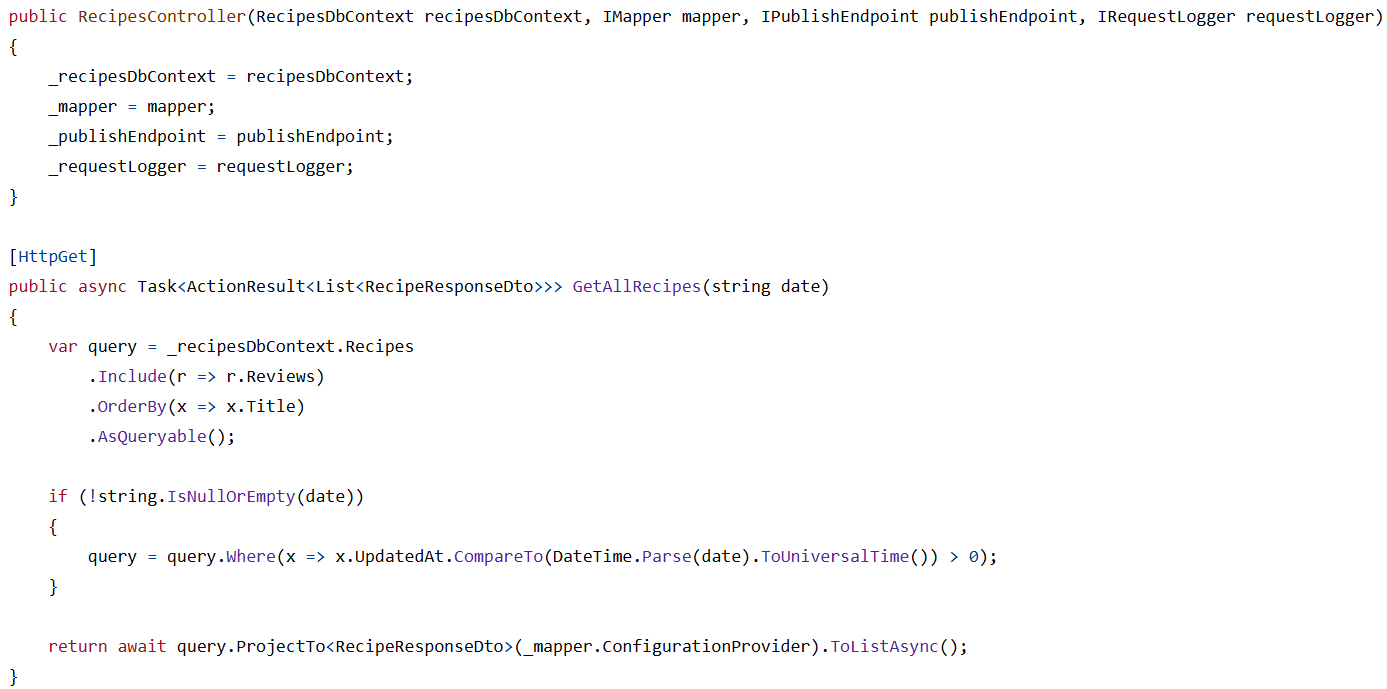
\includegraphics[width=1\textwidth]{images/dotnet-example.png}
    \caption{.NET API example.}
    \label{fig:dotnet-example}
\end{figure}
What about using LCOM and other modularity metrics on a web API application? LCOM is a metric that can be used to evaluate how well a module or a class fit's together. The use of frameworks might lead to some interesting class usage patterns, but the metrics can still be applied and in some cases give useful insight. For example when applied to a controller class in most cases the LCOM metric would give 0, because most methods in a controller share at least one dependency injection. LCOM above 0 might indicate that the controller class groups together end-points that shouldn't be grouped. The instability in normal controller usage should always be equal to 1, as controllers should not be used by other classes, having a lower instability metric might indicate miss-use of controller pattern. Similar analysis could be done for other class patterns like: data transfer classes, model classes, database context classes, etc. 
\newpage


\section{Container Criteria}
A container, according to the C4 model is the smallest separately deployable unit. Software systems are made up of containers. There are many types of containers. For example a server side web application, a database, a client side app, a shell script, etc. Some containers, such as a server side web application are built using code. Other containers, such as a database image, are bought (and later managed using SQL). Containers are kind of like a software system in the sense that they have to deliver some functionality and uphold to some quality requirements. However in many cases one container on it's own can't deliver anything. For example a service API can't serve requests without a database container. Therefore, this section will rather focus on general container evaluation criteria, but the reader should be aware that some of the software system criteria described in the later section, could also be applied to containers.

\subsection{Architectural Decisions}
One of the first activities in the software development life cycle is creating the architecture of the system. Many important decisions regarding containers have to be made at this stage, such as: selecting the runtime for each container, choosing the database technology or coding language, orchestrating the role of each container and their interactions. These decisions can later impact every high-level system metric, such as: reliability, security, cost, performance, etc. Below the author derives four criteria for assessing containers:
\\\textbf{Technology Choice}\\
Choosing technology is hard \cite{Naz21}. There are many considerations that an architect has to take into account, such as: cost, licensing, maturity, documentation, etc. Once the choice is made, the system then has to be built around that technology. Even if at the time the decision made sense, as time goes on the technology might get outdated or be no longer supported, which could lead to high maintenance costs. When choosing or re-evaluating technology a trade-off analysis has to be done.
\begin{figure}[H]
    \centering
    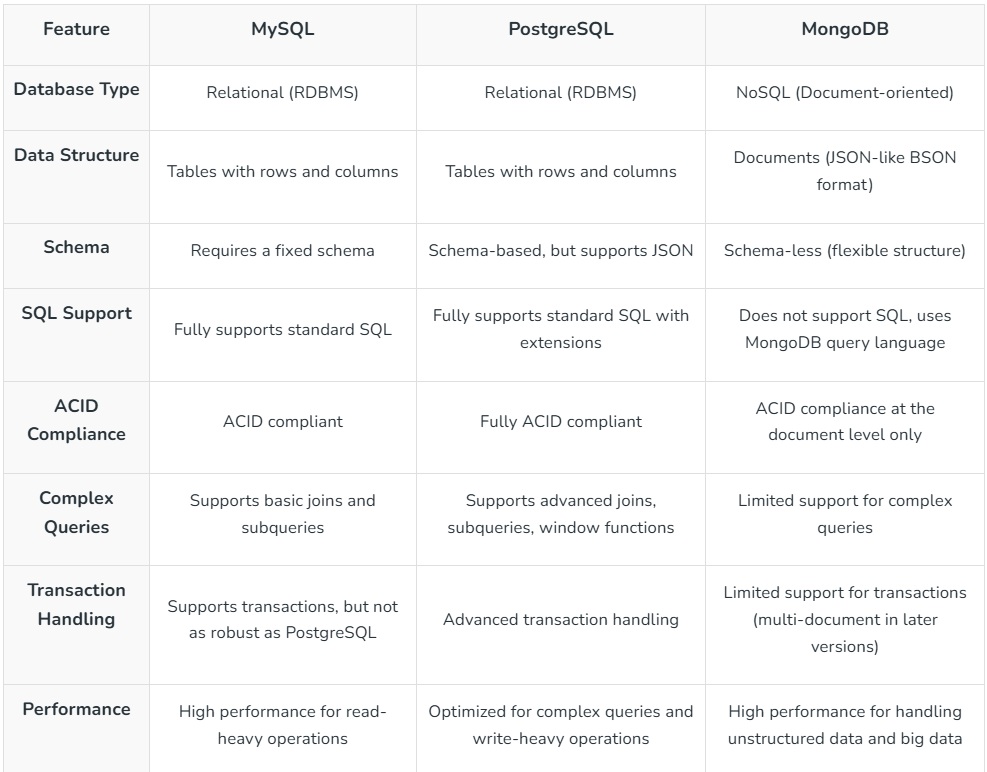
\includegraphics[width=1\textwidth]{images/technology-choice.png}
    \caption{Database technology comparison table from "geeksforgeeks" article.}
    \label{fig:technology-choice}
\end{figure}
Figure~\ref{fig:technology-choice} is a database technology comparison table from "geeksforgeeks" article. We can see that the choice can impact almost any architectural characteristic. For example choosing MongoDB might give us great performance on big data, but it wouldn't be functionally suitable for working with relational data. Or maybe if data quality was very important for us, we would choose an ACID compliant database.
\\\textbf{Deployment Environment}\\
A deployment environment is a combination of hardware and software systems, where the container is executed. For example:  your personal laptop with windows OS connected to a home network in Lithuania is a deployment environment, or a virtual machine in a mainframe computer, etc. Sometimes deployment is linked to technology choice. For example, Amazon Aurora database is only deployable on AWS cloud. The choice of deployment environment can greatly affect infrastructural cost and performance. A paper called "Cloud versus On-Premise Computing" by Cameron Fisher compares the costs of the cloud and on premises infrastructure \cite{Fis18}. The answer wether to go for cloud or on-premises depends on the use case. On-premises requires huge initial investments and IT staff to manage it. While cloud allows to get started immediately without any upfront costs. The paper ultimately finds that on premises approach can be cheaper in the long run with stable and predictable work loads. However, cloud offers many other benefits, such as edge computing and services that help build modern scalable applications.
\\\textbf{SRP}\\
The single responsibility principle might be one of the most important principles for designing clean distributed systems. A container should have a clearly defined purpose and boundaries. Containers that don't have a clear responsibility can be hard to use and make the system chaotic. Also a process that has multiple responsibilities is hard to scale, as one task might be memory intensive and another compute, etc.
\\\textbf{Documentation}\\
A container needs to have two things documented: it's interface and it's internal code. Having the interface well documented makes the container usable. While having, it's internal code documented makes it modifiable and maintainable. Metrics can be derived to measure the extent of documentation, such as the percentage of functions with doc-strings, however usually a simple assessment is enough.

\subsection{Operational Metrics}
A deployed container in C4 terms is a container instance. We can use simple metrics like: CPU usage, network usage, memory and disk usage to get early warning signs, that the system's performance may degrade soon. Other metrics like throughput usually require interactions between multiple container instances.

\subsection{Test Coverage}
Previously covered modularity metrics work great for evaluating individual code pieces (modules), but what about metrics that cover the whole container. While it is possible to derive the average values for the previous metrics, those would likely not provide much insight into the quality of the system. \par
One of the most important parts of software system life cycle is testing. Various different testing types exist for different purposes. For example, system tests are great for verifying the functionality and quality characteristics of a system, it helps answer the question: does the system do what it's intended to do? However, system testing is not the only type of testing. Unit tests are smaller tests that are written to verify the functionality of a small portion of the code like a class or a method. Test coverage is a metric that measures the portion of the code that gets executed when the unit tests are run.
\begin{figure}[H]
    \centering
    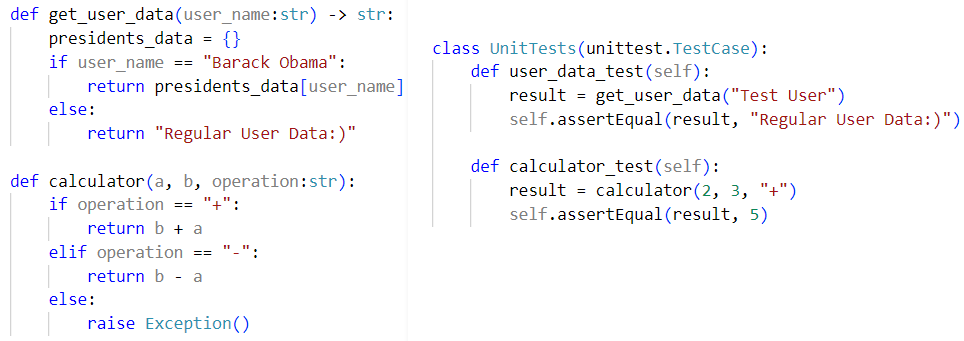
\includegraphics[width=1\textwidth]{images/python-code-coverage.png}
    \caption{Code coverage example.}
    \label{fig:python-code-coverage}
\end{figure}
Figure~\ref{fig:python-code-coverage} shows two functions that both have a mistake in one of the branches of the flow. "get\_user\_data" will end up raising an exception, when input is "Barack Obama" and "calculator" has a logical error when calculating subtraction. Both of these functions have a test written for them that covers only the correct part (76\% in total). Increasing the code coverage, in this case, would immediately reveal one of the bugs. High test coverage makes the system more reliable, it allows to catch bugs in the code, before going into production. Test coverage also makes the development more agile, by allowing developers to immediately see mistakes in new code or changes.

\subsection{Code Analysis}
Early identification of security issues and bugs in software development process can help increase the security and reliability of a container. Code review process is used widely in the software development world to help minimize the chance of vulnerabilities and bugs making to production. However the manual code reviews take a lot of human effort. Static application security testing tools (SASTs) automatically check the code for vulnerabilities based on predefined rules. A paper called "An Empirical Study of Static Analysis Tools for Secure Code Review" by Wachiraphan Charoenwet, Patanamon Thongtanunam, Van-Thuan Pham and Christoph Treude evaluates the accuracy of SASTs on real world vulnerability-contributing commits \cite{CTP24}. Their findings reveal that a single static application security test can detect 52\% of vulnerability containing functions. Also, when combining multiple SAST tools they were able to produce warnings for 78\% of vulnerability containing functions. That means that if your developers made one vulnerability contributing commit that could potentially lead to huge business losses, employing SASTs in software creation process would give you a 78\% chance of that never happening.


\subsection{API Quality Criteria}
Many modern software systems expose them self's through a REST API container. A well designed REST API increases the usability and quality of a container. An architect trying to assess the API design should compare it to a standard. Microsoft has released a great article on how to design RESTful APIs called "RESTful web API design" \cite{Mic23}. The article can be used as a reference to assess how well the API is designed.
\newpage


\section{System Level Metrics}
The highest level of abstraction in C4 model is a software system. Software system is a product of many container instances working together to deliver 'something'. Organizations don't invest in software just for the sake of it. That 'something' is usually described as a set of requirements. Organizations tend to split requirements into functional and non-functional. An example of a high level functional requirement could be: "Users of the system must be able to create an account and log in". An example of a non-functional requirement could be: "The system must have a 99.9999\% of up time". Evaluating the functionality of a system is usually a matter of answering a yes or no question. However non-functional system qualities are much more nuanced and therefore harder to evaluate.

\subsection{Existing Software Quality Models}
Software quality models help organizations understand what quality characteristics are relevant for their systems. Quality models define quality characteristics and sub characteristics that can be used as a reference, during requirements specification or when assessing an existing product. These models help the 'business side' stakeholders, however they do not define criteria and metrics for actually evaluating these characteristics. In Figure~\ref{fig:quality-models-comparison} a paper by Ming-Chang Lee called "Software Quality Factors and Software Quality Metrics to Enhance Software Quality Assurance" compares a few existing models \cite{Lee14}.
\begin{figure}[H]
    \centering
    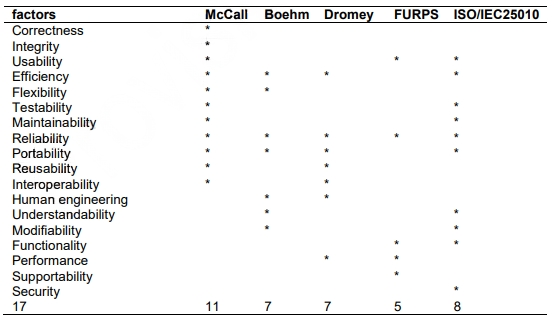
\includegraphics[width=0.6\textwidth]{images/quality-models-comparison.png}
    \caption{Software quality models comparison \cite{Lee14}.}
    \label{fig:quality-models-comparison}
\end{figure}
Many quality characteristics like: maintainability, efficiency, and reliability are shared between the models. The models also define sub-quality characteristics. For example, ISO/IEC 25010 relates maturity, fault tolerance, recover-ability, availability to reliability quality characteristic. In the end all of these quality models cover the whole scope of a software system.

\subsection{Turning Quality Factors Into System Tests}
Evaluating quality characteristics and sub-characteristics is not a trivial task. Business side stakeholders might ask for "a very reliable system", but how do you actually know if a system is reliable? This subsection will focus on ways to turn quality characteristics into tests or actionable criteria.
\subsubsection{Functional Suitability}
\textbf{Binary Functionality Evaluation}\\
Evaluating the functionality of a system is usually a matter of answering a yes or no question. For example, if one of the requirements was that: users should be able to leave comments, we could verify that by going into the website and trying to leave a comment. This process can be automated using functional tests. 
\\\textbf{Custom Accuracy Metrics}\\
Some systems require a more nuanced evaluation than simply answering a yes or no question. For example search engines will always return a result when the user submit's a query, however some results are better than the others. Figure~\ref{fig:search-results} compares Google and Bing results for the same search query. We can see that the two results are quite different. But one of the results will be more relevant to the user.
\begin{figure}[H]
    \centering
    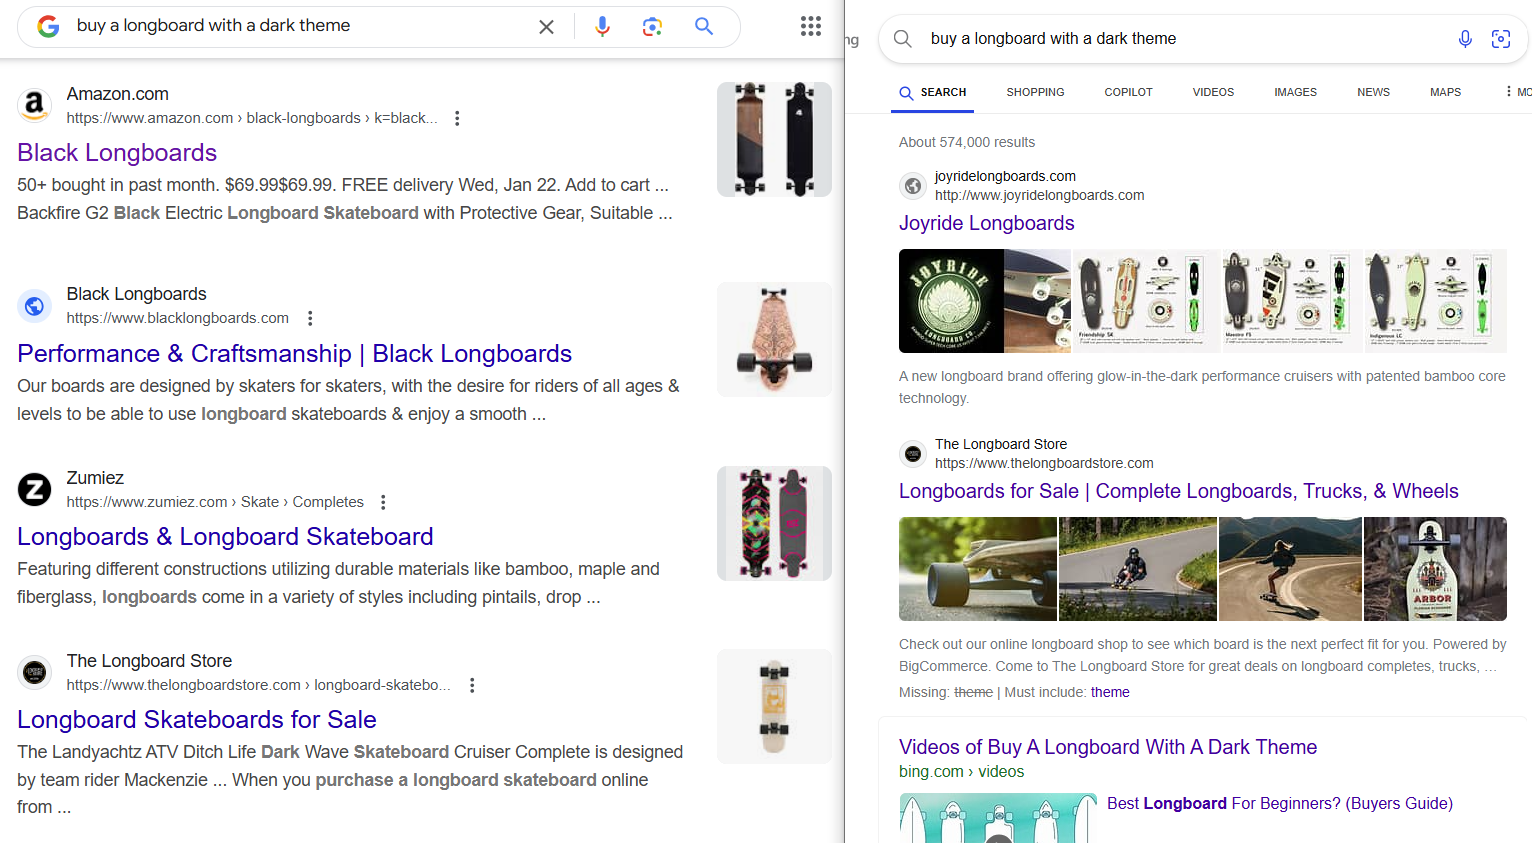
\includegraphics[width=0.6\textwidth]{images/search-results.png}
    \caption{Google \& Bing search results comparison.}
    \label{fig:search-results}
\end{figure}
Many problem questions can be raised here, such as: how can the two results be compared? Is it possible to give a score to each result? Is it possible to ultimately score a search system?
An example of a custom metric that could help compare the results is relevant websites count. By counting the amount of relevant links in both Google and Bing results we could effectively compare them. According to a Medium article by Jim Tao called "How to Evaluate Search Engines" we could take this a step further and calculate the precision and recall metrics \cite{Tao19}.
\[
\text{Precision} = \frac{| \text{Rel} \cap \text{Res} |}{| \text{Res} |}
\]

\[
\text{Recall} = \frac{| \text{Rel} \cap \text{Res} |}{| \text{Rel} |}
\]
Rel - here is the set of all relevant results to a query and res is the set of returned results by the engine. While these metrics are a good start, they lie on the assumption that relevance is binary and don't take into account the ordering. Furthermore, to this kind of analysis a set of query and relevant results pairs needs to be defined. Then the system can be evaluated similar to how a machine learning model is - by checking it's performance on a test set. Another way to examine a query result is by looking at user behavior. By accumulating user behavior on a search query we can create a 'click-through curve', that measures how many times on which item the users clicked. These metrics can further be used with other statistical techniques to improve the search engine's performance. \par
Note, that custom accuracy metrics can differ highly for each domain, but statistical methods will likely be involved when defining them.
\subsubsection{Performance Efficiency}
In ISO/IEC 25010 performance efficiency refers to how well can a system perform with certain resources. \textbf{Response Time} and \textbf{Throughput} are the two traditionally used metrics for evaluating system's performance. Response time measures the amount of time from the initiation of request till the response is received. Throughput measures the number of requests that a system can handle in a given time frame. To fully evaluate performance efficiency, we also need to take into account the resources used, which ultimately come down to \textbf{Infrastructure Cost}. Public cloud providers usually have cost calculators which can be used to compare different architecture costs.
\subsubsection{Other Quality Characteristics}
So far the author has covered 2 out of 8 quality characteristics defined by ISO/IEC 25010. The other quality characteristics are: Reliability, Operability, Security, Compatibility, Maintainability, Portability. Defining system level metrics and criteria for the later 6 quality characteristics is out of scope for this term paper. However, metrics and criteria defined in the container and modularity sections affect all of the quality characteristics. For example, as described in the containers section, employing SAST tools can help catch up to 78\% of vulnerability contributing commits, which positively affects security quality characteristic. In the results and conclusion section the author relates all of the ISO/IEC 25010 quality characteristics to metrics and criteria covered in this term paper.
% \subsection{System Structure}
\newpage %------MAIN CONTENT END------%

    
\section*{Results and Conclusion} %------RESULTS & CONCLUSION------%
\addcontentsline{toc}{section}{Results and Conclusion}
The author has covered a broad range of metrics and criteria that can be used to assess software systems in various scenarios. Cyclomatic complexity, LCOM and other modularity metrics are applicable to modern programming frameworks. Modularity metrics are best used as indicators, to spot potentially troublesome parts of code, rather than to assess it. Structural system properties like: container technology choice, deployment environment, segregation of duties and API design require manual evaluation methods, to determine wether they are suitable or not. Quality (sub)characteristics are just abstract properties of a system and their value is heavily influenced by the criteria and metrics covered in this paper. For example, test coverage and static code analysis are proven techniques that help increase reliability and security by revealing bugs and vulnerabilities early. Quality characteristics are too abstract to be evaluated directly, however system level metrics can be established to get a good sense of quality characteristics. For example functional suitability can be evaluated using binary functional tests and custom accuracy metrics. 'Custom accuracy metrics' term was derived to capture all non-binary functionality evaluation. \par
In Table 1 the author provides a summary of all metrics and criteria covered in this term paper. Each metric/criteria is associated with a quality characteristic from the ISO/IEC 25010 software product quality model and a C4 level. ISO/IEC 25010 connects the metrics and criteria to the 'business side', while the C4 model helps architects get a sense of what the metric/criteria is about. While this table covers a good chunk of most relevant criteria and metrics, this is certainly not an exhaustive list and a lot more research would have to be done to make this into a useful framework. Potential area of improvement is structuring the metrics even further, for example based on wether they are: operational, indicative, evaluate suitability, etc.

% Operational vs non-operational vs indicative vs suitability evaluation vs ... ?
\begin{figure}[H]
    \centering
    \captionsetup{labelformat=empty}
    \caption{Table 1: Software architecture assessment framework}
    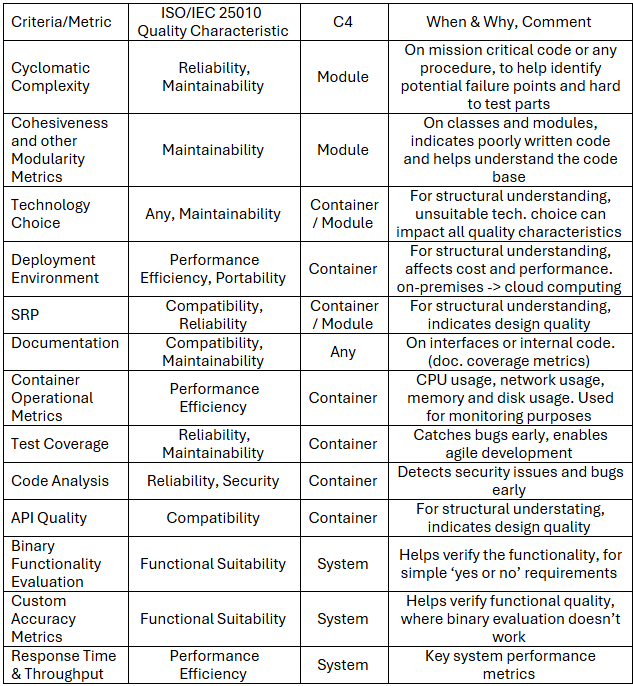
\includegraphics[width=1\textwidth]{images/results-table.png}
    \label{tab:results-table}
\end{figure}
% turi būti aiškiai išdėstomi pagrindiniai darbo rezultatai (kažkas
% išanalizuota, kažkas sukurta, kažkas įdiegta) ir pateikiamos išvados (daromi nagrinėtų problemų
% sprendimo metodų palyginimai, teikiamos rekomendacijos, akcentuojamos naujovės).
\newpage %------RESULTS & CONCLUSION END------%


% \section*{Sources} %------SOURCES PAGE------%
\addcontentsline{toc}{section}{References}
%%%%%%%%% Example 2%%%%%%%%%%%%%%%%%%%%%%%
\begin{thebibliography}{100}
\addtolength{\leftmargin}{0.2in}
    \setlength{\itemindent}{-0.2in}

    \bibitem[RF20]{RF20} M. Richards, N. Ford \emph{Fundamentals of Software Architecture: An Engineering Approach}, 2020.
    \bibitem[Bro11]{Bro11} S. Brown \emph{C4 Model}, Link access: \url{https://c4model.com/}. Viewed at: 2025-01-16.
    \bibitem[Mcc76]{Mcc76} T. J. McCabe \emph{Cyclomatic Complexity Wikipedia Article}, Link access: \url{https://en.wikipedia.org/wiki/Cyclomatic_complexity}. Viewed at: 2025-01-16.
    \bibitem[Naz21]{Naz21} S. Nazeer \emph{Choosing Technologies As An Architect}, Link access: \url{https://medium.com/codex/choosing-technologies-as-an-architect-8284a661f6a4}. Viewed at: 2025-01-16.
    \bibitem[Fis18]{Fis18} C. Fisher \emph{Cloud versus On-Premise Computing}, 2018, Link access: \url{https://www.scirp.org/journal/paperinformation?paperid=87661}. Viewed at: 2025-01-16.
    \bibitem[CTP24]{CTP24} W. Charoenwet, P. Thongtanunam, V. T. Pham and C. Treude \emph{An Empirical Study of Static Analysis Tools for Secure Code Review}, 2024, Link access: \url{https://dl.acm.org/doi/pdf/10.1145/3650212.3680313}. Viewed at: 2025-01-16.
    \bibitem[Mic23]{Mic23} Microsoft \emph{RESTful web API design}, 2023, Link access: \url{https://learn.microsoft.com/en-us/azure/architecture/best-practices/api-design}. Viewed at: 2025-01-16.
    \bibitem[Lee14]{Lee14} M. C. Lee \emph{Software Quality Factors and Software Quality Metrics to Enhance Software Quality Assurance}, 2014.
    \bibitem[Mar15]{Mar15} R. Martin \emph{Object-oriented metrics}, 2015, Link access: \url{https://kariera.future-processing.pl/blog/object-oriented-metrics-by-robert-martin/}. Viewed at: 2025-01-16.
    \bibitem[Tao19]{Tao19} J. Tao \emph{How to Evaluate Search Engines}, 2019, Link access: \url{https://medium.com/@jianbao.tao/how-to-evaluate-search-engines-b29e0a11a342}. Viewed at: 2025-01-16.
\end{thebibliography}
%%%%%%%%%% end %%%%%%%%%%%%%%%%%%%%%%%%%%
\newpage %------SOURCES PAGE END------%


\end{document}